\documentclass[12pt,a4paper]{article}

% ─── Page Layout ───────────────────────────────────────────────────────────────
\usepackage[a4paper, margin=0.8in, headheight=14pt]{geometry}

% ─── Fonts (XeLaTeX) ───────────────────────────────────────────────────────────
\usepackage{fontspec}
\usepackage{unicode-math}
\setmainfont{TeX Gyre Pagella}
\setmonofont[Scale=0.88]{TeX Gyre Cursor}
\setmathfont{Latin Modern Math}

% ─── Packages ──────────────────────────────────────────────────────────────────
\usepackage{xcolor}
\usepackage{colortbl}
\usepackage{titlesec}
\usepackage{enumitem}
\usepackage{tabularx}
\usepackage{booktabs}
\usepackage{array}
\usepackage{amsmath}
\usepackage{tikz}
\usetikzlibrary{shapes.geometric, arrows.meta, positioning, calc, fit, decorations.pathreplacing, patterns}
\usepackage{tcolorbox}
\tcbuselibrary{skins, breakable}
\usepackage{hyperref}
\usepackage{fancyhdr}
\usepackage{graphicx}
\usepackage{microtype}
\hyphenpenalty=10000
\exhyphenpenalty=10000
\sloppy
\usepackage{caption}
\usepackage{setspace}
\usepackage{multirow}
\usepackage{tocloft}

% ─── Q&A helper ────────────────────────────────────────────────────────────────
\newcommand{\Q}[1]{\textbf{#1}\par\noindent\ignorespaces}

% ─── Colour Palette ────────────────────────────────────────────────────────────
\definecolor{myred}{RGB}{196,30,58}
\definecolor{mydark}{RGB}{30,30,50}
\definecolor{mygreen}{RGB}{14,120,80}
\definecolor{myteal}{RGB}{0,130,140}
\definecolor{myamber}{RGB}{180,100,0}
\definecolor{mypurple}{RGB}{100,30,160}
\definecolor{mygray}{RGB}{246,247,249}
\definecolor{mgframe}{RGB}{180,185,200}
\definecolor{watermark}{RGB}{145,150,170}
\definecolor{hdrred}{RGB}{250,232,235}
\definecolor{hdrgreen}{RGB}{220,244,233}
\definecolor{hdrteal}{RGB}{220,242,244}
\definecolor{hdramber}{RGB}{253,242,215}
\definecolor{hdrpurple}{RGB}{238,228,255}
\definecolor{hdrgray}{RGB}{238,240,245}
\definecolor{rowalt}{RGB}{250,251,253}

% ─── Section Formatting ────────────────────────────────────────────────────────
\titleformat{\section}
  {\large\bfseries\color{myred}}{\thesection.}{0.5em}{}
  [\vspace{1pt}{\color{myred}\rule{\linewidth}{0.8pt}}]
\titleformat{\subsection}
  {\normalsize\bfseries\color{myteal}}{\thesubsection}{0.5em}{}
\titlespacing*{\section}{0pt}{18pt}{7pt}
\titlespacing*{\subsection}{0pt}{11pt}{4pt}

% ─── Paragraph ─────────────────────────────────────────────────────────────────
\setlength{\parindent}{0pt}
\setlength{\parskip}{4pt}

% ─── TOC Styling ───────────────────────────────────────────────────────────────
\renewcommand{\cfttoctitlefont}{\large\bfseries\color{myred}}
\renewcommand{\cftaftertoctitle}{\par\noindent{\color{myred}\rule{\linewidth}{0.8pt}}}
\setlength{\cftbeforetoctitleskip}{0pt}
\setlength{\cftaftertoctitleskip}{6pt}
\renewcommand{\cftsecfont}{\normalsize\bfseries\color{mydark}}
\renewcommand{\cftsecpagefont}{\normalsize\bfseries\color{mydark}}
\renewcommand{\cftsecleader}{\cftdotfill{\cftdotsep}}
\setlength{\cftbeforesecskip}{7pt}
\renewcommand{\cftsubsecfont}{\small\color{mydark}}
\renewcommand{\cftsubsecpagefont}{\small\color{mydark}}
\setlength{\cftbeforesubsecskip}{3pt}
\setlength{\cftsubsecindent}{1.4em}

% ─── Table helpers ─────────────────────────────────────────────────────────────
\renewcommand{\arraystretch}{1.45}
\setlength{\tabcolsep}{6pt}
\arrayrulecolor{mydark}
\newcolumntype{B}[1]{>{\small\bfseries\raggedright\arraybackslash}m{#1}}
\newcolumntype{Y}{>{\small\raggedright\arraybackslash}X}
\renewcommand{\tabularxcolumn}[1]{m{#1}}

% ─── Header / Footer ───────────────────────────────────────────────────────────
\pagestyle{fancy}
\fancyhf{}
\fancyhead[L]{\small\color{myred}\textbf{BS-M301}\;\color{mydark}--- Probability and Statistics}
\fancyhead[R]{\small\color{myteal}\textbf{Module 5 Notes}}
\fancyfoot[C]{\small\color{mydark}\thepage}
\fancyfoot[R]{\small\color{watermark}\textit{\copyright\ Biraj}}
\renewcommand{\headrulewidth}{0.5pt}
\renewcommand{\footrulewidth}{0.3pt}

% ─── Hyperref ──────────────────────────────────────────────────────────────────
\hypersetup{
  colorlinks=true, linkcolor=myteal, urlcolor=myteal,
  pdfauthor={Biraj Sarkar (CGEC)},
  pdftitle={BS-M301 --- Module 5 Notes: Applied Statistics, Curve Fitting and Tests of Significance}
}

% ─── tcolorbox styles ──────────────────────────────────────────────────────────
\tcbset{
  tikzbox/.style={
    colback=mygray, colframe=mgframe, boxrule=0.6pt, arc=4pt,
    left=8pt, right=8pt, top=6pt, bottom=6pt,
    colbacktitle=mgframe, coltitle=mydark,
    fonttitle=\small\bfseries
  },
  defbox/.style={
    colback=hdrgreen, colframe=mygreen, boxrule=0.8pt, arc=4pt,
    left=9pt, right=9pt, top=6pt, bottom=6pt,
    colbacktitle=mygreen, coltitle=white,
    fonttitle=\small\bfseries
  },
  formulabox/.style={
    colback=hdrteal, colframe=myteal, boxrule=0.8pt, arc=4pt,
    left=9pt, right=9pt, top=7pt, bottom=7pt,
    colbacktitle=myteal, coltitle=white,
    fonttitle=\small\bfseries
  },
  examplebox/.style={
    colback=hdramber, colframe=myamber, boxrule=0.8pt, arc=4pt,
    left=9pt, right=9pt, top=6pt, bottom=6pt,
    colbacktitle=myamber, coltitle=white,
    fonttitle=\small\bfseries
  },
  masonbox/.style={
    colback=hdrpurple, colframe=mypurple, boxrule=0.8pt, arc=4pt,
    left=9pt, right=9pt, top=6pt, bottom=6pt,
    colbacktitle=mypurple, coltitle=white,
    fonttitle=\small\bfseries
  },
  exambox/.style={
    colback=hdrpurple, colframe=mypurple, boxrule=1pt, arc=5pt,
    left=10pt, right=10pt, top=8pt, bottom=8pt,
    colbacktitle=mypurple, coltitle=white,
    fonttitle=\bfseries,
    breakable, title after break={\textbf{Frequently Asked / Viva Questions (contd.)}}
  }
}
\tcbset{breakable}
\tcbset{after={\color{black}}}

% ─── TikZ styles ───────────────────────────────────────────────────────────────
\tikzset{
  arrow/.style={-Stealth, thick, color=mydark},
  redarrow/.style={-Stealth, thick, color=myred},
  line/.style={thick, color=mydark}
}

\begin{document}

% ─── Title Page ───────────────────────────────────────────────────────────────
\begin{center}
  {\LARGE\bfseries\color{myred} BS-M301 --- Probability and Statistics}\\[5pt]
  {\normalsize\color{mydark} Semester III \quad$\bullet$\quad 3L:0T:3P \quad$\bullet$\quad 3 Credits}\\[3pt]
  {\normalsize\color{myteal}\textbf{Module 5 Exam Notes: Applied Statistics, Curve Fitting and Tests of Significance}}\\[3pt]
  {\small\color{mydark} CGEC \;$|$\; B.Tech ECE (2023--27) \;$|$\; \textit{Biraj Sarkar}}
\end{center}
\vspace{2pt}
\noindent{\color{myred}\rule{\linewidth}{1.5pt}}
\vspace{2pt}

\hypersetup{linkcolor=mydark}
\tableofcontents
\hypersetup{linkcolor=myteal}
\newpage

% ───────────────────────────────────────────────────────────────────────────────
\section{Curve Fitting by the Method of Least Squares}
% ───────────────────────────────────────────────────────────────────────────────

In experimental electronics and engineering measurement, observational data points $(x_1, y_1), (x_2, y_2), \dots, (x_n, y_n)$ rarely lie on an exact mathematical curve due to sensor noise and environmental fluctuations. The \textbf{Method of Least Squares} provides an objective criterion to establish the best-fitting functional relationship $y = f(x; a, b, c, \dots)$ by minimizing the sum of the squared vertical discrepancies.

\begin{tcolorbox}[defbox, title={\textbf{Definition: The Principle of Least Squares}}]
Let $(x_i, y_i)$ be $n$ paired experimental measurements. For any chosen curve $y = f(x)$, the residual (vertical error) for the $i$-th observation is:
\begin{equation}
  e_i = y_i - f(x_i)
\end{equation}
The Principle of Least Squares states that the optimal curve parameters are those that minimize the total sum of squared residuals:
\begin{equation}
  S = \sum_{i=1}^n e_i^2 = \sum_{i=1}^n \left[y_i - f(x_i; a, b, c, \dots)\right]^2 = \text{Minimum}
\end{equation}
To achieve this minimum, the partial derivatives of $S$ with respect to each undetermined parameter must vanish simultaneously:
\begin{equation}
  \frac{\partial S}{\partial a} = 0, \qquad \frac{\partial S}{\partial b} = 0, \qquad \frac{\partial S}{\partial c} = 0, \quad \dots
\end{equation}
The resulting system of simultaneous equations is called the \textbf{Normal Equations}.
\end{tcolorbox}

\begin{tcolorbox}[tikzbox, title={\textbf{TikZ Schematic: Residual Errors and Best-Fit Curve in Least Squares}}]
\begin{center}
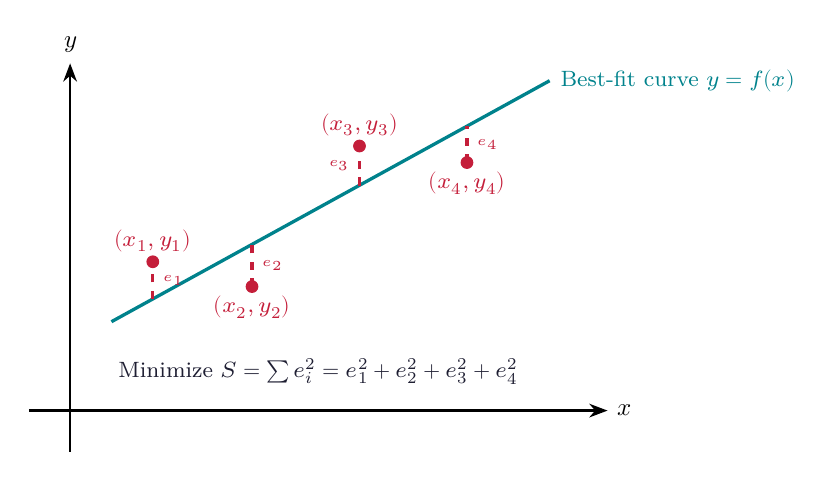
\begin{tikzpicture}[scale=1.05, every node/.style={font=\small}]
  % Axes
  \draw[-Stealth, thick] (-0.5, 0) -- (6.5, 0) node[right] {$x$};
  \draw[-Stealth, thick] (0, -0.5) -- (0, 4.2) node[above] {$y$};

  % Best fit line y = 0.55x + 0.8
  \draw[very thick, color=myteal] (0.5, 1.075) -- (5.8, 3.99) node[right, font=\footnotesize] {Best-fit curve $y = f(x)$};

  % Sample data points and vertical residuals
  % p1 = (1.0, 1.8), line = 1.35, e1 = +0.45
  \filldraw[color=myred] (1.0, 1.8) circle (2pt) node[above, font=\footnotesize] {$(x_1, y_1)$};
  \draw[dashed, very thick, color=myred] (1.0, 1.35) -- (1.0, 1.8) node[midway, right, font=\tiny] {$e_1$};

  % p2 = (2.2, 1.5), line = 2.01, e2 = -0.51
  \filldraw[color=myred] (2.2, 1.5) circle (2pt) node[below, font=\footnotesize] {$(x_2, y_2)$};
  \draw[dashed, very thick, color=myred] (2.2, 1.5) -- (2.2, 2.01) node[midway, right, font=\tiny] {$e_2$};

  % p3 = (3.5, 3.2), line = 2.72, e3 = +0.48
  \filldraw[color=myred] (3.5, 3.2) circle (2pt) node[above, font=\footnotesize] {$(x_3, y_3)$};
  \draw[dashed, very thick, color=myred] (3.5, 2.72) -- (3.5, 3.2) node[midway, left, font=\tiny] {$e_3$};

  % p4 = (4.8, 3.0), line = 3.44, e4 = -0.44
  \filldraw[color=myred] (4.8, 3.0) circle (2pt) node[below, font=\footnotesize] {$(x_4, y_4)$};
  \draw[dashed, very thick, color=myred] (4.8, 3.0) -- (4.8, 3.44) node[midway, right, font=\tiny] {$e_4$};

  % Caption
  \node[above, color=mydark, font=\footnotesize] at (3.0, 0.2) {Minimize $S = \sum e_i^2 = e_1^2 + e_2^2 + e_3^2 + e_4^2$};
\end{tikzpicture}
\end{center}
\end{tcolorbox}

\subsection{1. Fitting of a Straight Line: $y = a + bx$}
\begin{tcolorbox}[examplebox, title={\textbf{Derivation of Normal Equations for a Straight Line}}]
Let the straight line equation be $y = a + bx$. The error sum of squares is:
\begin{equation}
  S = \sum_{i=1}^n (y_i - a - bx_i)^2
\end{equation}
Differentiating partially with respect to $a$ and equating to zero:
\begin{align}
  \frac{\partial S}{\partial a} &= \sum_{i=1}^n 2(y_i - a - bx_i)(-1) = 0 \implies \sum_{i=1}^n (y_i - a - bx_i) = 0 \nonumber \\[3pt]
                                &\implies \sum y = n a + b \sum x
\end{align}
Differentiating partially with respect to $b$ and equating to zero:
\begin{align}
  \frac{\partial S}{\partial b} &= \sum_{i=1}^n 2(y_i - a - bx_i)(-x_i) = 0 \implies \sum_{i=1}^n x_i (y_i - a - bx_i) = 0 \nonumber \\[3pt]
                                &\implies \sum x y = a \sum x + b \sum x^2
\end{align}
\textbf{The Normal Equations for a Straight Line:}
\begin{align}
  \sum y &= n a + b \sum x \\[3pt]
  \sum x y &= a \sum x + b \sum x^2
\end{align}
\textit{Computation Shortcut (Change of Origin):} If $n$ is odd and values of $x$ are equally spaced, choosing the origin at the midpoint such that $\sum u = 0$ simplifies the solution to:
\begin{equation}
  a = \frac{\sum y}{n}, \qquad b = \frac{\sum u y}{\sum u^2}
\end{equation}
\end{tcolorbox}

\subsection{2. Fitting of a Second-Degree Parabola: $y = a + bx + cx^2$}
\begin{tcolorbox}[formulabox, title={\textbf{Normal Equations for a Second-Degree Parabola}}]
For the quadratic curve $y = a + bx + cx^2$, the sum of squared errors is $S = \sum (y_i - a - bx_i - cx_i^2)^2$.
Setting $\frac{\partial S}{\partial a} = 0, \frac{\partial S}{\partial b} = 0, \frac{\partial S}{\partial c} = 0$ yields the $3 \times 3$ system of \textbf{Normal Equations}:
\begin{align}
  \sum y &= n a + b \sum x + c \sum x^2 \\[4pt]
  \sum x y &= a \sum x + b \sum x^2 + c \sum x^3 \\[4pt]
  \sum x^2 y &= a \sum x^2 + b \sum x^3 + c \sum x^4
\end{align}
When origin is shifted to make $\sum u = 0$ (which also implies $\sum u^3 = 0$ for symmetric spacing):
\begin{align}
  \sum y &= n a + c \sum u^2 \\[2pt]
  \sum u y &= b \sum u^2 \implies b = \frac{\sum u y}{\sum u^2} \\[2pt]
  \sum u^2 y &= a \sum u^2 + c \sum u^4
\end{align}
\end{tcolorbox}

\subsection{3. Fitting of Non-Linear / General Curves via Linearization}
Many non-linear physical relationships can be linearized by taking logarithms:
\par\vspace{6pt}\noindent
\begingroup
\setlength{\tabcolsep}{5pt}
\setlength{\extrarowheight}{3pt}
\begin{tabularx}{\linewidth}{|B{3.2cm}|B{3.5cm}|B{3.2cm}|Y|}
\hline
\textbf{Curve Model} & \textbf{Log Transformation} & \textbf{Transformed Form} & \textbf{Normal Equations} \\
\hline
Exponential Curve \newline $y = a e^{bx}$ & $\ln y = \ln a + bx$ & $Y = A + bx$ \newline ($Y = \ln y, A = \ln a$) & $\sum Y = n A + b \sum x$ \newline $\sum x Y = A \sum x + b \sum x^2$ \\
\hline
Power / Geometric \newline $y = a x^b$ & $\log_{10} y = \log_{10} a + b \log_{10} x$ & $Y = A + b X$ \newline ($Y=\log y, X=\log x$) & $\sum Y = n A + b \sum X$ \newline $\sum X Y = A \sum X + b \sum X^2$ \\
\hline
Modified Exponential \newline $y = a b^x$ & $\log y = \log a + x \log b$ & $Y = A + B x$ \newline ($A=\log a, B=\log b$) & $\sum Y = n A + B \sum x$ \newline $\sum x Y = A \sum x + B \sum x^2$ \\
\hline
Hyperbolic Curve \newline $y = \frac{a}{x} + b$ & Substitute $u = \frac{1}{x}$ & $y = a u + b$ & $\sum y = a \sum u + n b$ \newline $\sum u y = a \sum u^2 + b \sum u$ \\
\hline
\end{tabularx}
\endgroup
\vspace{12pt}

% ───────────────────────────────────────────────────────────────────────────────
\section{Foundations of Statistical Hypothesis Testing}
% ───────────────────────────────────────────────────────────────────────────────

\begin{tcolorbox}[defbox, title={\textbf{Definition: Terminology of Statistical Testing}}]
\begin{enumerate}[leftmargin=*, itemsep=2pt, topsep=2pt]
  \item \textbf{Statistical Hypothesis:} An assertion or conjecture concerning the unknown parameter(s) of a population distribution.
  \item \textbf{Null Hypothesis ($H_0$):} The baseline hypothesis of \textit{no effect}, \textit{no difference}, or \textit{status quo}. It is maintained until evidence indicates otherwise.
  \item \textbf{Alternative Hypothesis ($H_1$):} The mutually exclusive claim that contradicts $H_0$. It can be \textbf{two-tailed} ($H_1: \theta \ne \theta_0$) or \textbf{one-tailed} ($H_1: \theta > \theta_0$ or $H_1: \theta < \theta_0$).
  \item \textbf{Errors in Hypothesis Testing:}
  \begin{itemize}[leftmargin=*, itemsep=1pt]
    \item \textbf{Type I Error ($\alpha$):} Rejecting $H_0$ when $H_0$ is actually true (Producer's risk / False positive).
    \begin{equation}
      P(\text{Type I Error}) = \alpha = \text{Level of Significance}
    \end{equation}
    \item \textbf{Type II Error ($\beta$):} Failing to reject $H_0$ when $H_0$ is actually false (Consumer's risk / False negative).
    \item \textbf{Power of the Test ($1 - \beta$):} Probability of correctly rejecting a false null hypothesis.
  \end{itemize}
  \item \textbf{Critical Region (Rejection Region):} The set of values of the test statistic for which $H_0$ is rejected.
\end{enumerate}
\end{tcolorbox}

\begin{tcolorbox}[tikzbox, title={\textbf{TikZ Schematic: Standard Normal Test Statistic with Two-Tailed Critical Regions ($\alpha = 0.05$)}}]
\begin{center}
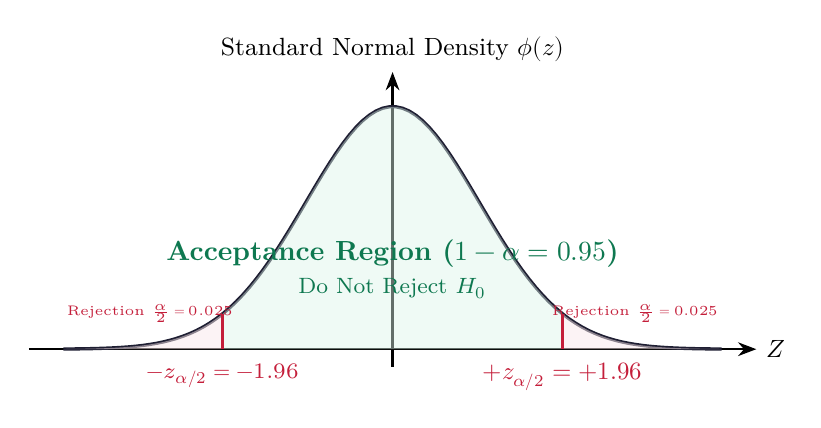
\begin{tikzpicture}[scale=1.1, every node/.style={font=\small}]
  % Axes
  \draw[-Stealth, thick] (-4.2, 0) -- (4.2, 0) node[right] {$Z$};
  \draw[-Stealth, thick] (0, -0.2) -- (0, 3.2) node[above] {Standard Normal Density $\phi(z)$};

  % Bell curve
  \draw[very thick, color=mydark, domain=-3.8:3.8, samples=100]
    plot (\x, {2.8*exp(-(\x)^2/2)});

  % Acceptance region (center)
  \fill[fill=hdrgreen, fill opacity=0.45, domain=-1.96:1.96, samples=60]
    (-1.96,0) -- plot (\x, {2.8*exp(-(\x)^2/2)}) -- (1.96,0) -- cycle;
  \node[color=mygreen, font=\bfseries] at (0, 1.1) {Acceptance Region ($1 - \alpha = 0.95$)};
  \node[color=mygreen, font=\footnotesize] at (0, 0.7) {Do Not Reject $H_0$};

  % Left critical tail (Z < -1.96)
  \fill[fill=hdrred, fill opacity=0.5, domain=-3.8:-1.96, samples=40]
    (-3.8,0) -- plot (\x, {2.8*exp(-(\x)^2/2)}) -- (-1.96,0) -- cycle;
  \draw[very thick, color=myred] (-1.96, 0) -- (-1.96, 0.41);
  \node[below, color=myred, font=\footnotesize] at (-1.96, -0.05) {$-z_{\alpha/2} = -1.96$};
  \node[above, color=myred, font=\tiny] at (-2.8, 0.2) {Rejection $\frac{\alpha}{2} = 0.025$};

  % Right critical tail (Z > +1.96)
  \fill[fill=hdrred, fill opacity=0.5, domain=1.96:3.8, samples=40]
    (1.96,0) -- plot (\x, {2.8*exp(-(\x)^2/2)}) -- (3.8,0) -- cycle;
  \draw[very thick, color=myred] (1.96, 0) -- (1.96, 0.41);
  \node[below, color=myred] at (1.96, -0.05) {$+z_{\alpha/2} = +1.96$};
  \node[above, color=myred, font=\tiny] at (2.8, 0.2) {Rejection $\frac{\alpha}{2} = 0.025$};
\end{tikzpicture}
\end{center}
\end{tcolorbox}

\subsection{Critical Values for Large Sample Tests ($Z$-Distribution)}
\par\vspace{6pt}\noindent
\begingroup
\setlength{\tabcolsep}{6pt}
\setlength{\extrarowheight}{3pt}
\begin{tabularx}{\linewidth}{|B{3.0cm}|B{3.2cm}|B{3.5cm}|Y|}
\hline
\textbf{Level of Significance ($\alpha$)} & \textbf{Two-Tailed Critical Value ($|Z| > z_{\alpha/2}$)} & \textbf{Right-Tailed Critical Value ($Z > z_\alpha$)} & \textbf{Left-Tailed Critical Value ($Z < -z_\alpha$)} \\
\hline
$\alpha = 5\% \; (0.05)$ & $z_{0.025} = 1.96$ & $z_{0.05} = 1.645$ & $-z_{0.05} = -1.645$ \\
\hline
$\alpha = 1\% \; (0.01)$ & $z_{0.005} = 2.576$ & $z_{0.01} = 2.326$ & $-z_{0.01} = -2.326$ \\
\hline
$\alpha = 10\% \; (0.10)$ & $z_{0.05} = 1.645$ & $z_{0.10} = 1.282$ & $-z_{0.10} = -1.282$ \\
\hline
\end{tabularx}
\endgroup
\vspace{12pt}

% ───────────────────────────────────────────────────────────────────────────────
\section{Large Sample Tests of Significance ($Z$-Tests, $n \ge 30$)}
% ───────────────────────────────────────────────────────────────────────────────

By the Central Limit Theorem, for sample sizes $n \ge 30$, sample statistics (proportions, means, variances) are approximately normally distributed regardless of the underlying parent population distribution. The general test statistic is:
\begin{equation}
  Z = \frac{\text{Sample Statistic} - \text{Hypothesized Parameter Value}}{\text{Standard Error of the Statistic (SE)}} \sim \mathcal{N}(0, 1)
\end{equation}

\subsection{1. Large Sample Test for a Single Proportion}
Testing whether a population proportion $P$ equals a specified value $P_0$.
\begin{tcolorbox}[formulabox, title={\textbf{Test for Single Proportion}}]
\begin{itemize}[leftmargin=*, itemsep=2pt]
  \item \textbf{Hypotheses:} $H_0: P = P_0 \quad \text{vs} \quad H_1: P \ne P_0$ (two-tailed) or $P > P_0$ (right-tailed).
  \item \textbf{Sample Proportion:} $p = \frac{x}{n}$, where $x$ is the number of successes in $n$ trials.
  \item \textbf{Standard Error under $H_0$:} $\text{SE}(p) = \sqrt{\frac{P_0 Q_0}{n}}$, where $Q_0 = 1 - P_0$.
  \item \textbf{Test Statistic:}
  \begin{equation}
    Z = \frac{p - P_0}{\sqrt{\dfrac{P_0 Q_0}{n}}}
  \end{equation}
  \item \textbf{Decision Rule:} If $|Z| > 1.96$ (at $5\%$ level), reject $H_0$.
\end{itemize}
\end{tcolorbox}

\subsection{2. Large Sample Test for Difference of Two Proportions}
Testing whether two independent populations have identical success proportions ($P_1 = P_2$).
\begin{tcolorbox}[formulabox, title={\textbf{Test for Difference of Two Proportions}}]
\begin{itemize}[leftmargin=*, itemsep=2pt]
  \item \textbf{Hypotheses:} $H_0: P_1 = P_2 \quad \text{vs} \quad H_1: P_1 \ne P_2$.
  \item \textbf{Sample Proportions:} $p_1 = \frac{x_1}{n_1}$ and $p_2 = \frac{x_2}{n_2}$.
  \item \textbf{Pooled Proportion Estimate (under $H_0$):}
  \begin{equation}
    \hat{p} = \frac{x_1 + x_2}{n_1 + n_2} = \frac{n_1 p_1 + n_2 p_2}{n_1 + n_2}, \qquad \hat{q} = 1 - \hat{p}
  \end{equation}
  \item \textbf{Test Statistic:}
  \begin{equation}
    Z = \frac{p_1 - p_2}{\sqrt{\hat{p}\hat{q}\left(\dfrac{1}{n_1} + \dfrac{1}{n_2}\right)}}
  \end{equation}
\end{itemize}
\end{tcolorbox}

\subsection{3. Large Sample Test for a Single Mean}
Testing whether a population mean $\mu$ equals a specified value $\mu_0$.
\begin{tcolorbox}[formulabox, title={\textbf{Test for Single Mean}}]
\begin{itemize}[leftmargin=*, itemsep=2pt]
  \item \textbf{Hypotheses:} $H_0: \mu = \mu_0 \quad \text{vs} \quad H_1: \mu \ne \mu_0$.
  \item \textbf{Sample Mean:} $\bar{x} = \frac{1}{n} \sum_{i=1}^n x_i$.
  \item \textbf{Test Statistic:}
  \begin{equation}
    Z = \frac{\bar{x} - \mu_0}{\sigma / \sqrt{n}}
  \end{equation}
  If the population standard deviation $\sigma$ is unknown, it is replaced by sample SD $s = \sqrt{\frac{1}{n}\sum(x_i - \bar{x})^2}$ (valid since $n \ge 30$):
  \begin{equation}
    Z = \frac{\bar{x} - \mu_0}{s / \sqrt{n}}
  \end{equation}
\end{itemize}
\end{tcolorbox}

\subsection{4. Large Sample Test for Difference of Two Means}
Testing whether two independent populations have equal means ($\mu_1 = \mu_2$).
\begin{tcolorbox}[formulabox, title={\textbf{Test for Difference of Two Means}}]
\begin{itemize}[leftmargin=*, itemsep=2pt]
  \item \textbf{Hypotheses:} $H_0: \mu_1 = \mu_2 \quad \text{vs} \quad H_1: \mu_1 \ne \mu_2$.
  \item \textbf{Test Statistic:}
  \begin{equation}
    Z = \frac{\bar{x}_1 - \bar{x}_2}{\sqrt{\dfrac{\sigma_1^2}{n_1} + \dfrac{\sigma_2^2}{n_2}}} \approx \frac{\bar{x}_1 - \bar{x}_2}{\sqrt{\dfrac{s_1^2}{n_1} + \dfrac{s_2^2}{n_2}}}
  \end{equation}
\end{itemize}
\end{tcolorbox}

\subsection{5. Large Sample Test for Difference of Standard Deviations}
Testing whether two populations have identical variability ($\sigma_1 = \sigma_2$).
\begin{tcolorbox}[formulabox, title={\textbf{Test for Difference of Two Standard Deviations}}]
For a sample of size $n$ drawn from a normal population, the sampling distribution of the sample standard deviation $s$ is asymptotically normal with mean $\sigma$ and standard error:
\begin{equation}
  \text{SE}(s) = \frac{\sigma}{\sqrt{2n}}
\end{equation}
\textbf{Test Statistic for $H_0: \sigma_1 = \sigma_2$:}
\begin{equation}
  Z = \frac{s_1 - s_2}{\sqrt{\dfrac{\sigma_1^2}{2n_1} + \dfrac{\sigma_2^2}{2n_2}}} \approx \frac{s_1 - s_2}{\sqrt{\dfrac{s_1^2}{2n_1} + \dfrac{s_2^2}{2n_2}}}
\end{equation}
\end{tcolorbox}

\newpage
% ===============================================================================
% MANDATORY QUICK REVISION PAGE
% ===============================================================================
\begin{center}
  {\large\bfseries\color{myred} Quick Revision --- Module 5}\\[1pt]
  {\small\color{mydark} Applied Statistics, Curve Fitting and Tests of Significance $|$ BS-M301}
\end{center}
\noindent{\color{myred}\rule{\linewidth}{1.0pt}}
\vspace{1pt}

\begin{tcolorbox}[formulabox, top=2pt, bottom=2pt, title={\textbf{Key Normal Equations and Large Sample $Z$-Test Formulas at a Glance}}]
\renewcommand{\arraystretch}{0.96}
\setlength{\tabcolsep}{3.5pt}
\begin{tabularx}{\linewidth}{B{3.8cm} X}
Line Normal Equations & $\sum y = n a + b \sum x, \quad \sum x y = a \sum x + b \sum x^2$ \\[0.2pt]
Parabola Normal Eqs. & $\sum y = n a + b\sum x + c\sum x^2, \; \sum xy = a\sum x + b\sum x^2 + c\sum x^3, \; \sum x^2 y = a\sum x^2 + b\sum x^3 + c\sum x^4$ \\[0.2pt]
Exponential Curve & $y = a e^{bx} \implies \ln y = \ln a + bx \implies Y = A + bx$ \\[0.2pt]
Power Curve & $y = a x^b \implies \log y = \log a + b \log x \implies Y = A + bX$ \\[0.2pt]
Single Proportion Test & $Z = \frac{p - P_0}{\sqrt{P_0 Q_0 / n}}, \quad Q_0 = 1 - P_0$ \\[0.2pt]
Two Proportions Test & $Z = \frac{p_1 - p_2}{\sqrt{\hat{p}\hat{q}(1/n_1 + 1/n_2)}}, \quad \hat{p} = \frac{n_1 p_1 + n_2 p_2}{n_1 + n_2}, \; \hat{q} = 1 - \hat{p}$ \\[0.2pt]
Single Mean Test & $Z = \frac{\bar{x} - \mu_0}{\sigma / \sqrt{n}} \approx \frac{\bar{x} - \mu_0}{s / \sqrt{n}}$ \\[0.2pt]
Two Means Test & $Z = \frac{\bar{x}_1 - \bar{x}_2}{\sqrt{\sigma_1^2/n_1 + \sigma_2^2/n_2}} \approx \frac{\bar{x}_1 - \bar{x}_2}{\sqrt{s_1^2/n_1 + s_2^2/n_2}}$ \\[0.2pt]
Standard Deviation SE & $\text{SE}(s) = \frac{\sigma}{\sqrt{2n}}, \quad Z = \frac{s_1 - s_2}{\sqrt{s_1^2/(2n_1) + s_2^2/(2n_2)}}$ \\[0.2pt]
Critical $Z$-Values & $\alpha = 5\%: |Z| = 1.96 \text{ (two-tailed)}, 1.645 \text{ (one-tailed)}; \quad \alpha = 1\%: |Z| = 2.576$ \\
\end{tabularx}
\end{tcolorbox}

\vspace{1pt}

\begin{tcolorbox}[defbox, top=2pt, bottom=2pt, title={\textbf{One-Line Definitions}}]
\begin{itemize}[leftmargin=*, itemsep=-0.5pt, topsep=0pt, parsep=0pt]
  \item \textbf{Least Squares Principle:} Criterion minimizing the sum of squared vertical residuals $\sum (y_i - f(x_i))^2$.
  \item \textbf{Normal Equations:} Set of simultaneous linear equations obtained by setting partial derivatives of error to zero.
  \item \textbf{Null Hypothesis ($H_0$):} Initial baseline claim stating no difference, no effect, or parameter equality.
  \item \textbf{Alternative Hypothesis ($H_1$):} The competing research claim adopted if sample evidence contradicts $H_0$.
  \item \textbf{Type I Error ($\alpha$):} Mistakenly rejecting a true null hypothesis (false positive; significance level).
  \item \textbf{Type II Error ($\beta$):} Incorrectly failing to reject a false null hypothesis (false negative).
  \item \textbf{Power of Test ($1 - \beta$):} Probability of correctly rejecting $H_0$ when the alternative $H_1$ is true.
  \item \textbf{Critical Region:} Subspace of test statistics leading to rejection of $H_0$ at significance level $\alpha$.
  \item \textbf{Standard Error (SE):} Standard deviation of the sampling distribution of a given sample statistic.
  \item \textbf{Pooled Proportion ($\hat{p}$):} Combined success rate $(x_1+x_2)/(n_1+n_2)$ under the null hypothesis of equality.
\end{itemize}
\end{tcolorbox}

\newpage

\begin{tcolorbox}[exambox, title={\textbf{Frequently Asked / Viva Questions (Part 1)}}]
\begin{enumerate}[topsep=0pt, label=\textbf{Q\arabic*.}, itemsep=3.2pt]
  \item \Q{State the Principle of Least Squares and explain why vertical errors are squared.}
  The principle minimizes $S = \sum e_i^2 = \sum (y_i - \hat{y}_i)^2$. Errors are squared because (1) positive and negative errors would otherwise cancel out ($\sum e_i = 0$), (2) squaring penalizes large outliers heavily, and (3) $S$ is continuously differentiable, yielding linear normal equations.

  \item \Q{How can the exponential curve $y = a b^x$ be fitted using the method of least squares?}
  Taking base-10 logarithms: $\log y = \log a + x \log b$. Defining $Y = \log y, A = \log a$, and $B = \log b$, the model becomes the linear form $Y = A + Bx$. Solving standard linear normal equations for $A$ and $B$, the parameters are recovered via $a = 10^A$ and $b = 10^B$.

  \item \Q{Distinguish between Type I Error and Type II Error in hypothesis testing.}
  Type I error ($\alpha$) occurs when a true null hypothesis $H_0$ is mistakenly rejected (false alarm). Type II error ($\beta$) occurs when a false null hypothesis is accepted (missed detection). Decreasing $\alpha$ for a fixed sample size increases $\beta$.

  \item \Q{Why can the normal distribution be used for large sample tests even if the population is non-normal?}
  By the Central Limit Theorem (CLT), the sampling distribution of the sample mean $\bar{x}$ (and sample proportions) approaches a normal distribution as sample size $n \ge 30$, irrespective of the shape of the parent population.

  \item \Q{What is the difference between a one-tailed test and a two-tailed test?}
  A two-tailed test investigates departures in either direction ($H_1: \mu \ne \mu_0$), placing critical area $\alpha/2$ in both tails. A one-tailed test investigates directional superiority or inferiority ($H_1: \mu > \mu_0$ or $\mu < \mu_0$), concentrating the entire critical area $\alpha$ in one tail.

  \item \Q{State the standard error of the sample standard deviation for a normal population.}
  For large samples drawn from a normal population, $\text{SE}(s) = \frac{\sigma}{\sqrt{2n}}$. It is used to test significance of variance differences across industrial production lines.

  \item \Q{Why do we pool the proportions $\hat{p} = \frac{n_1 p_1 + n_2 p_2}{n_1 + n_2}$ in the two-proportion test?}
  Under the null hypothesis $H_0: P_1 = P_2 = P$, both samples originate from a single population with common proportion $P$. Pooling gives the minimum-variance unbiased estimator of this common parameter.
\end{enumerate}
\end{tcolorbox}

\newpage

\begin{tcolorbox}[exambox, top=3pt, bottom=3pt, title={\textbf{Frequently Asked / Viva Questions (Part 2)}}]
\begin{enumerate}[topsep=0pt, label=\textbf{Q\arabic*.}, itemsep=1.8pt, start=8]
  \item \Q{What decision is made if the calculated test statistic is $Z_{\text{cal}} = 2.15$ at $5\%$ significance level?}
  For a two-tailed test at $\alpha = 5\%$, the critical boundary is $Z_{\text{crit}} = 1.96$. Since $|Z_{\text{cal}}| = 2.15 > 1.96$, the sample statistic falls in the critical rejection region. We reject the null hypothesis $H_0$ and conclude the observed difference is statistically significant.

  \item \Q{How does shifting the origin simplify fitting a parabola $y = a + bx + cx^2$?}
  If $x$ values are symmetrically spaced, shifting the origin to the center makes $\sum u = 0$ and $\sum u^3 = 0$. The normal equations decouple into $b = \sum uy / \sum u^2$, while $a$ and $c$ decouple from $b$ into an elementary $2 \times 2$ system, dramatically reducing computational effort.

  \item \Q{What is the Level of Significance ($\alpha$) and how is it related to the confidence level?}
  The level of significance $\alpha$ is the maximum tolerable probability of committing a Type I error. It is related to the confidence level $C$ by $C = (1 - \alpha) \times 100\%$. For example, an $\alpha = 0.05$ level of significance corresponds to a $95\%$ confidence level.
\end{enumerate}
\end{tcolorbox}

\vspace{2pt}

\begin{tcolorbox}[tikzbox, top=3pt, bottom=3pt, title={\textbf{Summary Matrix: Comprehensive Decision Table of Large Sample Significance Tests}}]
\par\vspace{1pt}\noindent
\begingroup
\setlength{\tabcolsep}{3.5pt}
\setlength{\extrarowheight}{1.0pt}
\renewcommand{\arraystretch}{1.12}
\begin{tabularx}{\linewidth}{|B{2.5cm}|B{3.5cm}|B{3.2cm}|Y|}
\hline
\textbf{Test Type} & \textbf{Null Hypothesis ($H_0$)} & \textbf{Standard Error (SE)} & \textbf{Test Statistic ($Z_{\text{cal}}$)} \\
\hline
Single Proportion & $H_0: P = P_0$ & $\sqrt{\frac{P_0 Q_0}{n}}$ & $Z = \frac{p - P_0}{\sqrt{P_0 Q_0 / n}}$ \\
\hline
Two Proportions & $H_0: P_1 = P_2$ & $\sqrt{\hat{p}\hat{q}\left(\frac{1}{n_1} + \frac{1}{n_2}\right)}$ & $Z = \frac{p_1 - p_2}{\sqrt{\hat{p}\hat{q}(1/n_1 + 1/n_2)}}, \quad \hat{p} = \frac{n_1 p_1 + n_2 p_2}{n_1 + n_2}$ \\
\hline
Single Mean & $H_0: \mu = \mu_0$ & $\frac{\sigma}{\sqrt{n}} \approx \frac{s}{\sqrt{n}}$ & $Z = \frac{\bar{x} - \mu_0}{s / \sqrt{n}}$ \\
\hline
Two Means & $H_0: \mu_1 = \mu_2$ & $\sqrt{\frac{s_1^2}{n_1} + \frac{s_2^2}{n_2}}$ & $Z = \frac{\bar{x}_1 - \bar{x}_2}{\sqrt{s_1^2/n_1 + s_2^2/n_2}}$ \\
\hline
Two Std. Deviations & $H_0: \sigma_1 = \sigma_2$ & $\sqrt{\frac{s_1^2}{2n_1} + \frac{s_2^2}{2n_2}}$ & $Z = \frac{s_1 - s_2}{\sqrt{s_1^2/(2n_1) + s_2^2/(2n_2)}}$ \\
\hline
\end{tabularx}
\endgroup
\end{tcolorbox}

\end{document}
